\documentclass[11pt, letterpaper]{memoir}
\usepackage{HomeworkStyle}

\begin{document}
	\begin{center}
		{\large	Quiz 12.3 -- Modern Materials}
	\end{center}
	{\large Name: \rule[-1mm]{4in}{.1pt} 
	
	\subsection*{Question 1}
  Of the ionic compounds below, which would you expect to have the highest and lowest lattice energy

  \noindent{\large \ch{NaCl} \hspace{2em} \ch{LiF} \hspace{2em} \ch{MgO} \hspace{2em} \ch{CaS}}

	\subsection*{Question 2}
  In the space below, draw a band diagram for each of the following materials:

  \noindent{\large Metal \hspace{4em} Semiconductor \hspace{4em} n-doped Semiconductor \hspace{2em} p-doped Semiconductor}

	\vspace{13em}
  \subsection*{Question 3}
  \noindent Below are the chemical structures of two monomers. Draw the structure each would form when polymerized, and classify each polymer as an \emph{addition} polymer or a \emph{condensation} polymer

  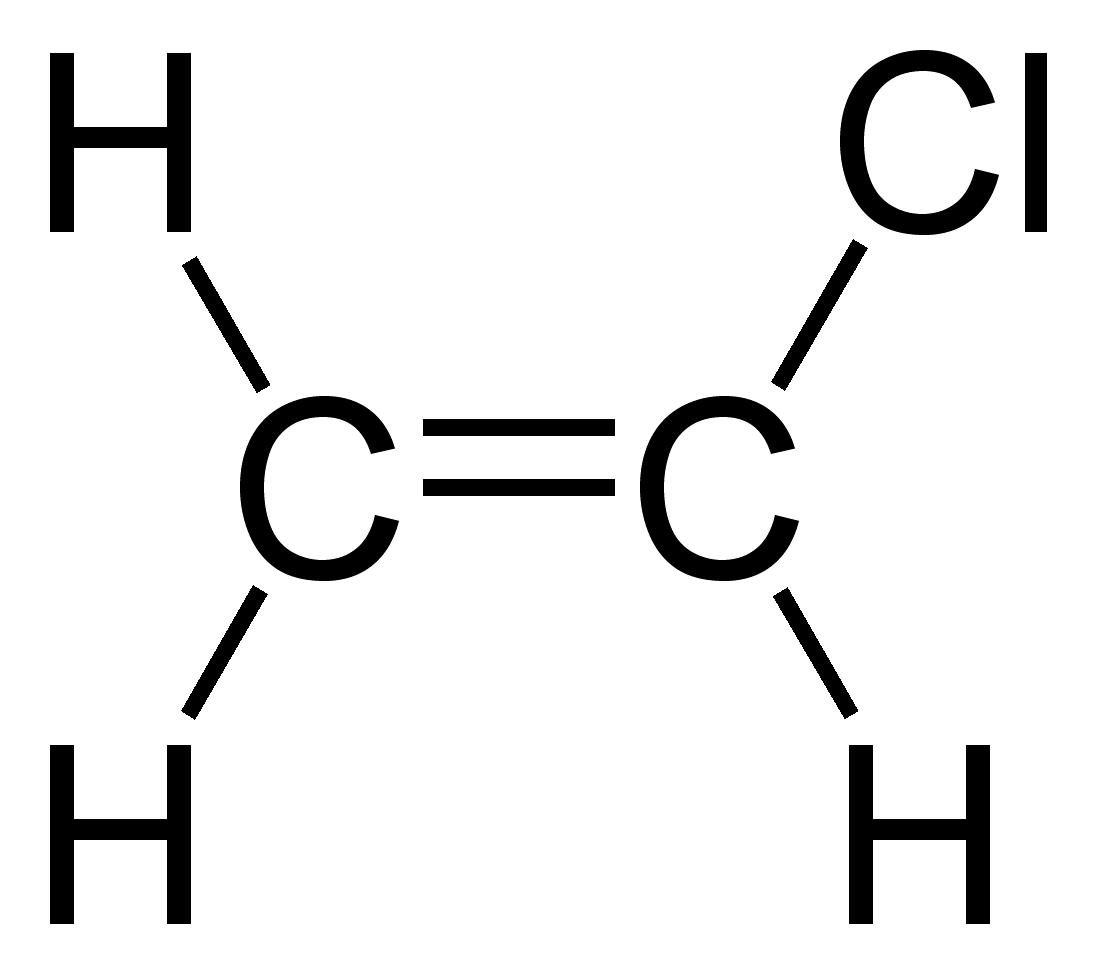
\includegraphics[scale=0.07]{vinyl_chloride.png} \hspace{15em} 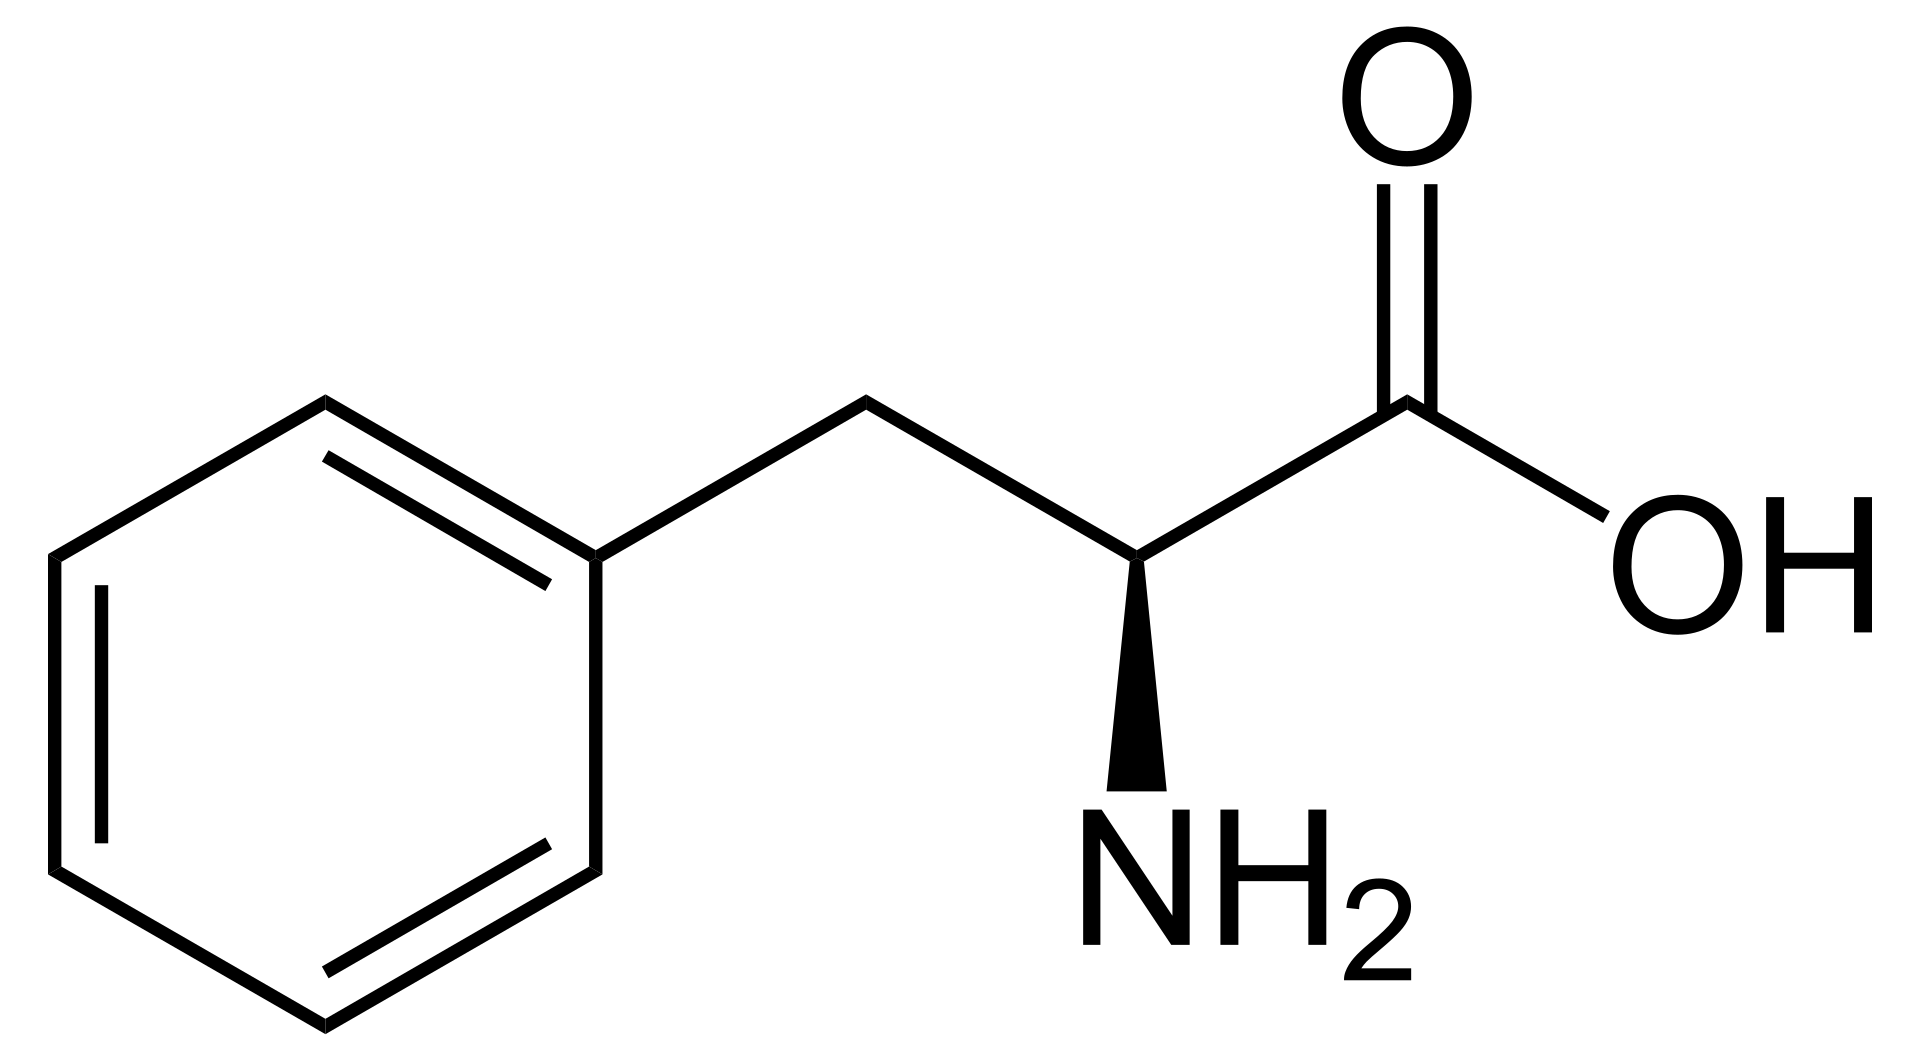
\includegraphics[scale=0.07]{phenylalinine.png}
	\newpage
	\pagestyle{empty}
	\addtocounter{page}{-1}
  \newgeometry{margin=1.25in}
  \section*{\emph{The Summer Day}}
  \paragraph{By Mary Oliver}~
  \begin{verse}
    Who made the world?\\
    Who made the swan, and the black bear?\\
    Who made the grasshopper?\\
    This grasshopper, I mean-\\
    the one who has flung herself out of the grass,\\
    the one who is eating sugar out of my hand,\\
    who is moving her jaws back and forth instead of up and down-\\
    who is gazing around with her enormous and complicated eyes.\\
    Now she lifts her pale forearms and thoroughly washes her face.\\
    Now she snaps her wings open, and floats away.\\
    I don't know exactly what a prayer is.\\
    I do know how to pay attention, how to fall down\\
    into the grass, how to kneel down in the grass,\\
    how to be idle and blessed, how to stroll through the fields,\\
    which is what I have been doing all day.\\
    Tell me, what else should I have done?\\
    Doesn't everything die at last, and too soon?\\
    Tell me, what is it you plan to do\\
    with your one wild and precious life?
  \end{verse}
\end{document}
